\documentclass[11pt]{article}

\usepackage[a4paper,hmargin=2.8cm,vmargin=2.6cm]{geometry}
\usepackage{titlesec}
\usepackage{mathtools}
\usepackage{listings}

\usepackage{graphicx}

\usepackage{biblatex}
\usepackage{hyperref}
\usepackage{cleveref}

\bibliography{tp2refs}

%% Set title

\title{\textit{Algorithms for speech and language processing}\\
{\sffamily TP2 Report: \textit{Building a probabilistic parser for French}}}

\author{Wilson Jallet}

\titleformat{\section}[hang]{\LARGE\bfseries\sffamily}{\thesection}{.5em}{}[]
\titleformat{\paragraph}[hang]{\large\bfseries\sffamily}{}{1em}{}[]

%% Set commands

\newcommand{\calN}{\mathcal{N}}
\newcommand{\calO}{\mathcal{O}}

\newcommand{\wer}{\mathrm{WER}}


\lstset{
	basicstyle=\sffamily,
	stringstyle=\sffamily,
	language=Python}

\begin{document}
\maketitle

\section{Implementation}

\paragraph{Building the PCFG and lexicon}

We split the treebank data in training and testing dataset, before shuffling the training data and re-splitting between training and validation. The shuffling is needed because lines in the treebank seem to be grouped together thematically\footnote{For instance l. 800--1000 discuss health, and l. 2700--2800 seem to discuss French politics.}. For reproducibility, we fixed the value of the random seed.

We use the Python Natural Language ToolKit (NLTK) \cite{nltkCitation} package to parse the treebank data as constituency trees in a way we can extract rules.
We then strip the lexical rules, leaving the part-of-speech (PoS) as terminals, and build the PCFG from these productions using the data structure provided in NLTK and a helper which computes the empirical probabilities of individual productions.

The lexical rules are transformed into a lexicon using our \lstinline|ProbabilisticLexicon| Python class, which holds the triples $(w,\mathrm{PoS}, p(\mathrm{PoS}|w))$ for every PoS and token $w$ (with nonzero probability) stored as a map $w \mapsto \{(\mathrm{PoS},p(\mathrm{PoS}|w))\}$.



\paragraph{Out-of-Vocabulary module}

There are two complementary strategies to propose surrogates for out-of-vocabulary (OOV) words: computing \textbf{spelling} nearest neighbors in the corpus according to the Levenshtein Edit distance, and computing \textbf{semantic} nearest neighbors according to the cosine distance of some embeddings (and intersecting with the corpus vocabulary).

For the Levenshtein-nearest neighbors, we run through the corpus and compute all the distances, and get the $k$ elements with the lowest distance (without sorting).
For the embedding nearest neighbors, we use Scikit-Learn's nearest neighbors implementation \cite{scikit-learn} (which is very efficient), which we fit using the cosine distance to measure semantic similarity\footnote{We actually use the Euclidean distance on normalized embedding vectors, which is equivalent to the cosine distance because $\|\frac{x}{\|x\|} - \frac{y}{\|y\|}\|^2 = 2 - 2\langle \frac{x}{\|x\|}, \frac{y}{\|y\|}\rangle$.}.

We run every input sentence through the module, which keeps in-corpus tokens and selects replacements for OOV words. The OOV module objective is to maximize the sum-total score under a language model trained on the corpus: we use NLTK to construct a unigram-bigram language model with a score function that averages between unigrams and bigrams (called Witten-Bell smoothing). The objective is solved using a greedy strategy: if $w_i$ is OOV, then its replacement $w'_i$ is the proposal that has the best individual score\footnote{Because the language model uses bigrams, it could also be possible to use a dynamic programming strategy and work backwards but this was not investigated.}.

\paragraph{CYK algorithm}

We implement a probabilistic version of the CYK algorithm, as explained on its Wikipedia page \cite{wiki:CYK}. Since the PCFG terminals are parts-of-speech, we integrate the words $w$ for the choice of PoS using the lexicon probabilities $p(\mathrm{PoS}|w)$.

\section{Results}


We evaluated our parser on the test dataset. We get the following results: out of 310 sentences, 82 failed to parse, and an average PoS tag accuracy of $86.0\%$.

We noticed a few problems. Handling OOV proper nouns is a difficult problem, especially when they are the first token in a sentence and thus have no context for the OOV module to use: it happens that common nouns or even verbs are used as replacements when they are picked up by edit distance, see \Cref{fig:npParseFailure_didiersoulage}.

\begin{figure}[ht!]
	\centering
	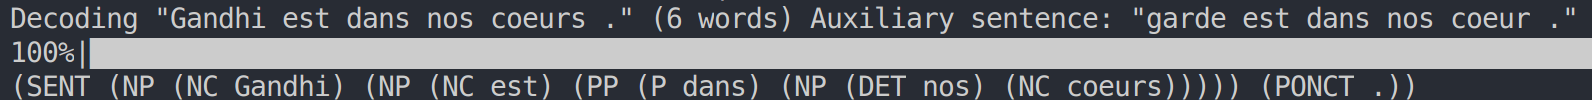
\includegraphics[width=\linewidth]{gandhi-garde.png}
	\caption{Failure of parsing a proper noun which is out-of-vocabulary.}
	\label{fig:npParseFailure_didiersoulage}
\end{figure}


\printbibliography{}


\end{document}